\chapter{BACKGROUND AND FUNDAMENTALS}\
\section{Brief QC Primer}
\hspace*{0.3in}Quantum Computing (QC) departs from the binary logic of classical systems by using qubits, which exist in superpositions of |0⟩ and |1⟩ states. Unlike classical bits, qubits can represent multiple possibilities simultaneously, enabling exponential growth in representational capacity with the number of qubits. Quantum gates, such as Hadamard (H), Pauli-X, and CNOT, manipulate qubit states by exploiting superposition and entanglement. These properties provide powerful mechanisms for parallelism but are extremely fragile. Error sources-including decoherence, gate imperfections, and environmental noise-pose a central challenge. Current devices rely heavily on error mitigation and correction strategies, such as surface codes, to maintain computational reliability.\\
\begin{figure}[htbp]
	\centering
	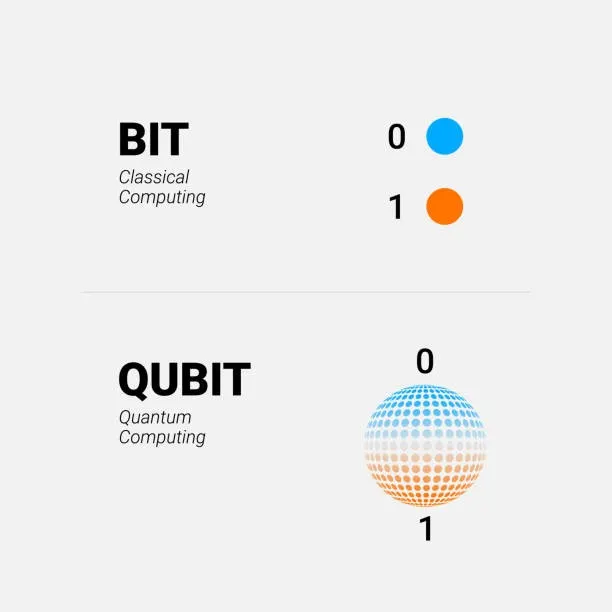
\includegraphics[width=0.6\linewidth]{qubit.png}
	\caption{Classical bits and Quantum bits}
	\label{fig:enter-label}
\end{figure}
\section{Brief AI/ML Primer}
\hspace*{0.3in}Artificial Intelligence (AI) broadly refers to systems capable of learning, reasoning, and decision-making. Within AI, Machine Learning (ML) enables computers to learn from data patterns rather than following explicit rules. ML methods span supervised, unsupervised, and semi-supervised paradigms. Deep Learning (DL)-driven by multi-layered neural networks-has revolutionized areas like computer vision and natural language processing. Another crucial branch, Reinforcement Learning (RL), focuses on agents that interact with environments to maximize long-term rewards. RL is particularly important for quantum contexts, as it supports adaptive control, calibration, and optimization tasks where environments are stochastic and high-dimensional.\\
\section{Hybrid Quantum-Classical Paradigms}
\hspace*{0.3in}The near-term reality of QC is shaped by Noisy Intermediate-Scale Quantum (NISQ) devices, which cannot yet perform fully error-free computations. To bridge this gap, hybrid quantum–classical paradigms have emerged. These combine quantum circuits for parts of a task (e.g., encoding large state spaces or sampling probability distributions) with classical algorithms for optimization, gradient updates, or post-processing. Well-known frameworks include the Variational Quantum Eigensolver (VQE) and the Quantum Approximate Optimization Algorithm (QAOA), where quantum subroutines are embedded within classical optimization loops. These paradigms illustrate how QC and AI can complement each other: quantum resources enhance exploration of complex spaces, while classical resources provide robustness and scalability.\\
\begin{figure}[htbp]
	\centering
	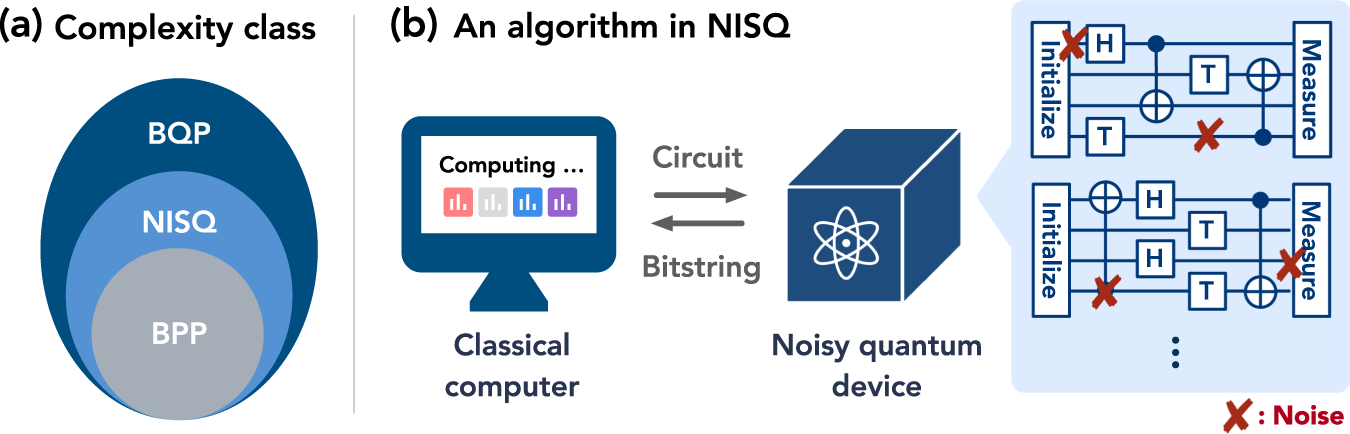
\includegraphics[width=1\linewidth]{nisq.png}
	\caption{Classical bits and Quantum bits}
	\label{fig:enter-label}
\end{figure}